\documentclass[10pt,aspectratio=169]{beamer}
%\documentclass[10pt]{beamer}

\usetheme[everytitleformat=regular]{m}

\usepackage{booktabs}
\usepackage[scale=2]{ccicons}

\usepackage{pgfplots}
\usepgfplotslibrary{dateplot}

\title{ESCAR 2015 USA}
\subtitle{Summary of Lectures}
\date{\today}
\author{Youngmin Kim}
\institute{Queensland University of Technology}
\titlegraphic{\hfill
\includegraphics[height=1.5cm]{img/qut-logo-og-200.jpg}}

\begin{document}

\maketitle

\begin{frame}
  \frametitle{Table of Contents}
  \setbeamertemplate{section in toc}[sections numbered]
  \tableofcontents[hideallsubsections]
\end{frame}

\section{Introduction}

\begin{frame}{Lists}
  \frametitle{What is ESCAR?}

  \begin{itemize}
      \item Embedded Security in CARs
      \item The leading automotive Cyber Security conference
      \item Free download service for Lectures
  \end{itemize}    
  \begin{figure}
      \centering
      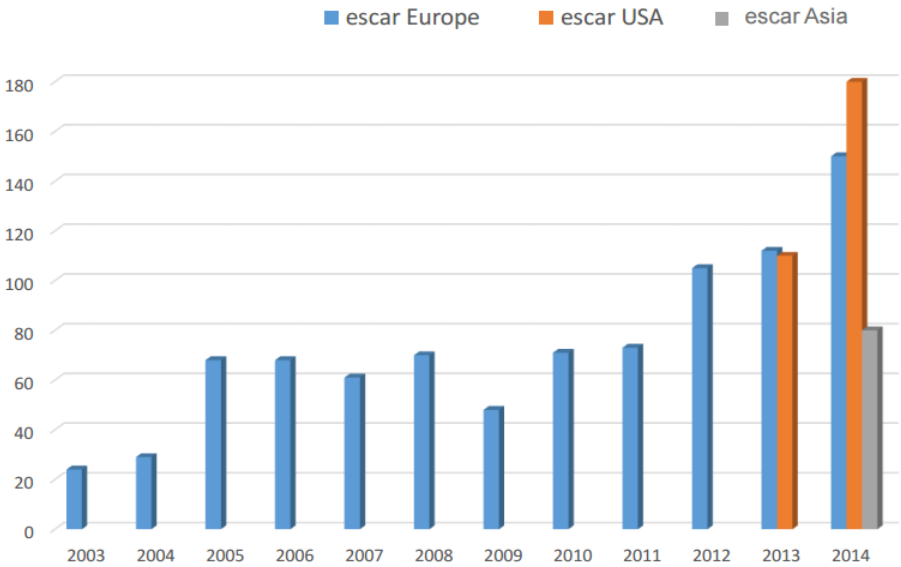
\includegraphics[trim={0 0 0 0},clip,scale=0.2]{img/participants.png} \caption{Participants}
  \end{figure}
\end{frame}

\begin{frame}{fragile}
  \frametitle{Areas of Call for Papers}

  {\small
  \begin{itemize}
      \item Security engineering, formal methods, development \& validation tools, 
          security standardization and security economics for automotive domain
      \item Security of vehicle-driven business, maintenance and service models
      \item Identity theft, privacy and data protection issues in vehicular settings
      \item Vehicular hardware security and hardware security modules
      \item Security of vehicular on-board, passenger, and V2X communications
      \item Security of software downloads and open vehicle application platforms
      \item Security of vehicular component protection solutions
      \item Security of legal car applications (e.g., event data recorder, tachograph)
      \item Security of road pricing, restricted areas access and vehicle monitoring
      \item Security of vehicle theft prevention and theft response solutions
      \item Security of vehicular rights control and audit (e.g., feature activation)
      \item Security of future vehicle applications (e.g., electric cars, ITS)
      \item Security for other transport systems (e.g., railways, aerospace)
  \end{itemize}
  }
\end{frame}

\begin{frame}{fragile}
  \frametitle{ESCAR 2015 USA Lectures}

  \begin{itemize}
      \item escar Europe 2014 -- Overview 12th escar Europe (Nov. 18-19, 2014)
  \end{itemize}
\end{frame}

\section{ESCAR Europe 2014 -- Overview}

\begin{frame}{fragile}
    \frametitle{Automotive Security Attacks (1/)}

    Overview of automotive pen-testing methods
    \begin{itemize}
        \item Search vulnerabilities
            \begin{itemize}
                \item Remote
                \item Firmware Extraction
                    \begin{itemize}
                        \item Extract data from the Flash chip
                        \item Debugger Port
                    \end{itemize}
            \end{itemize}
        \item Hacker's final goal is to control vechicle \textbf{through CAN bus}
        \item Example attack to \textbf{Zubie} Service
    \end{itemize}

    \begin{figure}
        \centering
        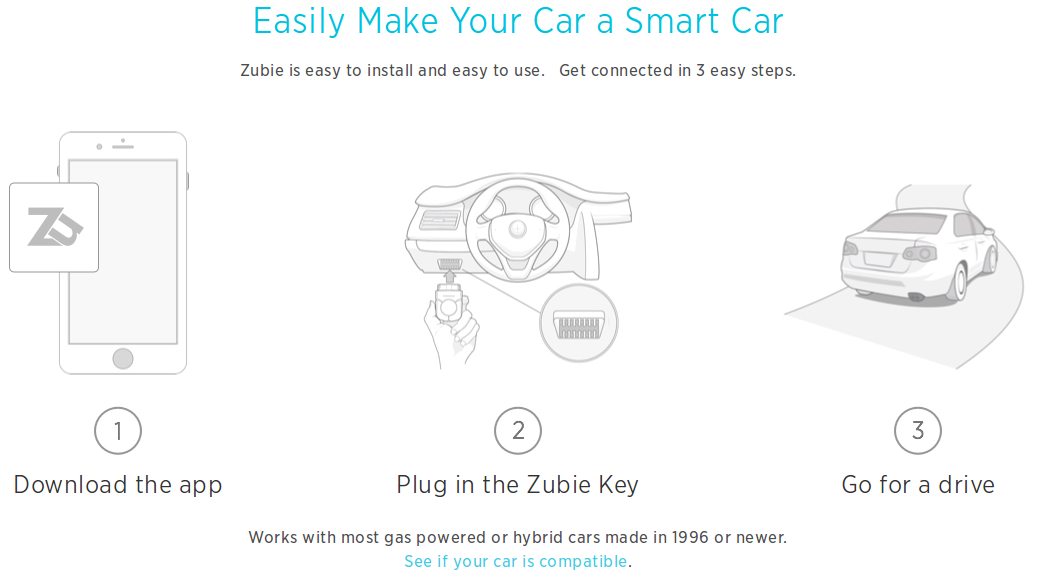
\includegraphics[trim={0 0 0 0},clip,scale=0.2]{img/zubie.png}
    \end{figure}
\end{frame}

\begin{frame}{fragile}
    \frametitle{Automotive Security Attacks (2/)}

    Demonstration of a False-data Injection Attack Against an FMCW Radar
    \begin{itemize}
        \item Search vulnerabilities
            \begin{itemize}
                \item Remote
                \item Firmware Extraction
                    \begin{itemize}
                        \item Extract data from the Flash chip
                        \item Debugger Port
                    \end{itemize}
            \end{itemize}
        \item Hacker's final goal is to control vechicle \textbf{through CAN bus}
        \item Example attack to \textbf{Zubie} Service
    \end{itemize}

\end{frame}


\section{Test-bed}


\section{Conclusion}

\begin{frame}{Summary}

  Get the source of this theme and the demo presentation from

  \begin{center}\url{github.com/matze/mtheme}\end{center}


  \begin{center}\ccbysa\end{center}

\end{frame}

\end{document}
